% This file was created by matplotlib2tikz v0.5.3.
% The lastest updates can be retrieved from
% 
% https://github.com/nschloe/matplotlib2tikz
% 
% where you can also submit bug reports and leavecomments.
% 
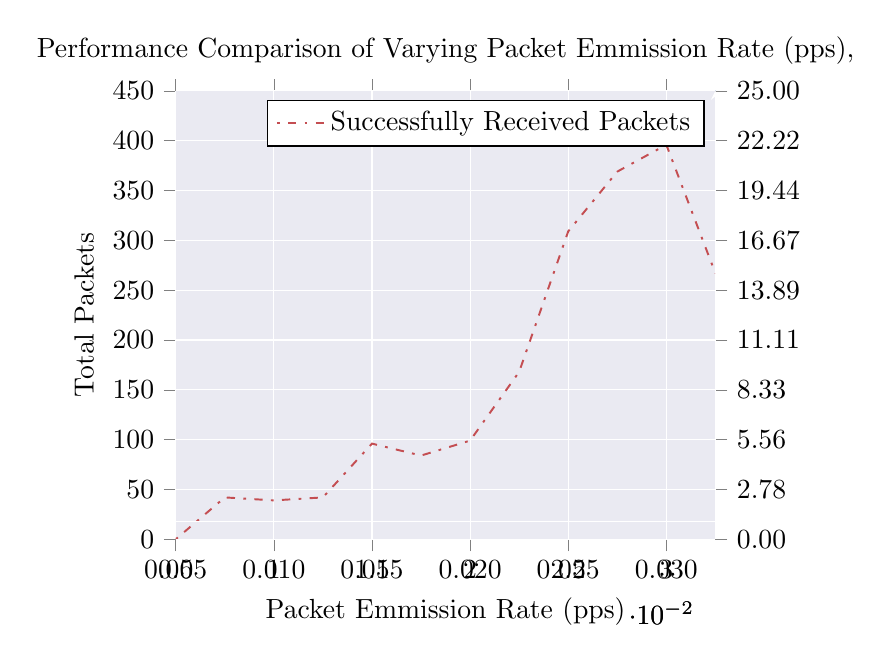
\begin{tikzpicture}

\definecolor{color1}{rgb}{0.298039215686275,0.447058823529412,0.690196078431373}
\definecolor{color0}{rgb}{0.917647058823529,0.917647058823529,0.949019607843137}
\definecolor{color3}{rgb}{0.768627450980392,0.305882352941176,0.32156862745098}
\definecolor{color2}{rgb}{0.333333333333333,0.658823529411765,0.407843137254902}

\begin{axis}[
title={Performance Comparison of Varying Packet Emmission Rate (pps),},
xlabel={Packet Emmission Rate (pps)},
ylabel={Total Packets},
xmin=0.005, xmax=0.0325,
ymin=0, ymax=450,
xtick={0.005,0.01,0.015,0.02,0.025,0.03,0.035},
xticklabels={$0.005$,$0.010$,$0.015$,$0.020$,$0.025$,$0.030$,},
ytick={0,50,100,150,200,250,300,350,400,450},
yticklabels={$0$,$50$,$100$,$150$,$200$,$250$,$300$,$350$,$400$,$450$},
tick align=outside,
xmajorgrids,
x grid style={white},
ymajorgrids,
y grid style={white},
axis line style={white},
axis background/.style={fill=color0},
legend entries={{Successfully Received Packets},{Enqueued Packets},{Collisions (right)}}
]
\addplot [line width=0.7000000000000001pt, color1]
table {%
0.005 90.3333333333333
0.0075 135.666666666667
0.01 180.166666666667
0.0125 224.333333333333
0.015 268.833333333333
0.0175 314.166666666667
0.02 358.833333333333
0.0225 403.5
0.025 442.333333333333
0.0275 426.833333333333
0.03 445.5
0.0325 449.5
};
\addplot [line width=0.7000000000000001pt, color2, dashed]
table {%
0.005 0
0.0075 0.166666666666667
0.01 0
0.0125 0.166666666666667
0.015 0.166666666666667
0.0175 0.166666666666667
0.02 0.166666666666667
0.0225 0.5
0.025 7.83333333333333
0.0275 71.5
0.03 94.5
0.0325 136
};
\path [draw=white, fill opacity=0] (axis cs:0.005,1)
--(axis cs:0.0325,1);

\path [draw=white, fill opacity=0] (axis cs:1,0)
--(axis cs:1,450);

\path [draw=white, fill opacity=0] (axis cs:0.005,0)
--(axis cs:0.0325,0);

\path [draw=white, fill opacity=0] (axis cs:0,0)
--(axis cs:0,450);

\end{axis}

\begin{axis}[
xmin=0.005, xmax=0.0325,
ymin=0, ymax=25,
axis y line=right,
ytick={0,2.77777777777778,5.55555555555556,8.33333333333333,11.1111111111111,13.8888888888889,16.6666666666667,19.4444444444444,22.2222222222222,25},
yticklabels={$0.00$,$2.78$,$5.56$,$8.33$,$11.11$,$13.89$,$16.67$,$19.44$,$22.22$,$25.00$},
tick align=outside,
xmajorgrids,
x grid style={white},
ymajorgrids,
y grid style={white},
axis line style={white},
axis background/.style={fill=color0},
legend entries={{Successfully Received Packets},{Enqueued Packets},{Collisions (right)}}
]
\addplot [line width=0.7000000000000001pt, color3, dash pattern=on 1pt off 3pt on 3pt off 3pt]
table {%
0.005 0
0.0075 2.33333333333333
0.01 2.16666666666667
0.0125 2.33333333333333
0.015 5.33333333333333
0.0175 4.66666666666667
0.02 5.5
0.0225 9.33333333333333
0.025 17.1666666666667
0.0275 20.5
0.03 22
0.0325 14.8333333333333
};
\path [draw=white, fill opacity=0] (axis cs:0.005,1)
--(axis cs:0.0325,1);

\path [draw=white, fill opacity=0] (axis cs:1,0)
--(axis cs:1,25);

\path [draw=white, fill opacity=0] (axis cs:0.005,0)
--(axis cs:0.0325,0);

\path [draw=white, fill opacity=0] (axis cs:0,0)
--(axis cs:0,25);

\end{axis}

\end{tikzpicture}